\documentclass[11pt]{article}
\usepackage[textwidth=18.0cm, textheight=23.0cm, top=2.0cm]{geometry}
\usepackage{pst-all}
\usepackage{amssymb}
\usepackage{tikz}
\usepackage{underscore}\begin{document}
\pagestyle{empty}


ClassName: \underline{\textbf{Class_06.2bp-12}}
\par
BinSize: \underline{\textbf{300 × 300}}
\par
ReduceSize: \underline{\textbf{300 × 300}}
\par
TypeNum: \underline{\textbf{40}}
\par
Num: \underline{\textbf{40}}
\par
OutS: \underline{\textbf{180000}}
\par
InS: \underline{\textbf{115372}}
\par
Rate: \underline{\textbf{0.641}}
\par
UB: \underline{\textbf{2}}
\par
LB0: \underline{\textbf{2}}
\par
LB: \underline{\textbf{2}}
\par
LBWithCut: \underline{\textbf{2}}
\par
NodeCut: \underline{\textbf{0}}
\par
ExtendedNodeCnt: \underline{\textbf{1}}
\par
GenNodeCnt: \underline{\textbf{1}}
\par
PrimalNode: \underline{\textbf{0}}
\par
ColumnCount: \underline{\textbf{2}}
\par
TotalCutCount: \underline{\textbf{0}}
\par
RootCutCount: \underline{\textbf{0}}
\par
LPSolverCnt: \underline{\textbf{1}}
\par
PricingSolverCnt: \underline{\textbf{0}}
\par
BranchAndBoundNum: \underline{\textbf{1}}
\par
isOpt: \underline{\textbf{true}}
\par
TimeOnPrimal: \underline{\textbf{0.000 s}}
\par
TimeOnPricing: \underline{\textbf{0.000 s}}
\par
TimeOnRmp: \underline{\textbf{0.078 s}}
\par
TotalTime: \underline{\textbf{0.156 s}}
\par
\newpage


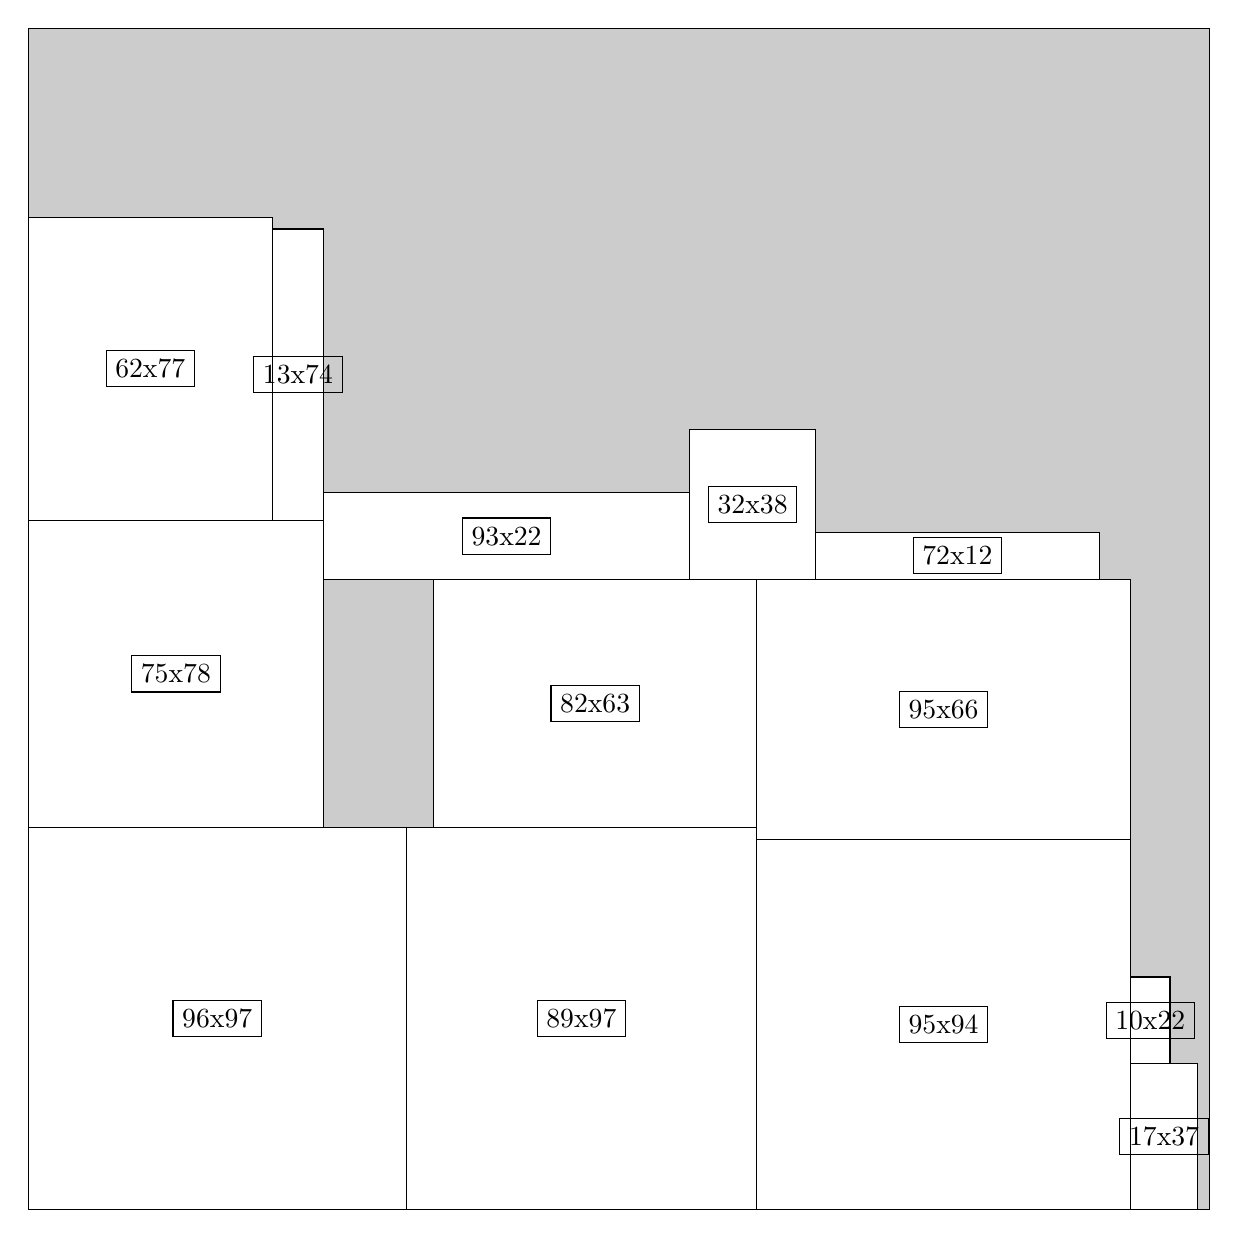
\begin{tikzpicture}[shorten >=1pt,scale=1.0,every node/.style={scale=1.0},->]
\tikzstyle{vertex}=[circle,fill=black!25,minimum size=14pt,inner sep=0pt]
\filldraw[fill=gray!40!white, draw=black] (0,0) rectangle (15.0,15.0);
\foreach \name/\x/\y/\w/\h in {96x97/0.0/0.0/4.800000000000001/4.8500000000000005,95x94/9.25/0.0/4.75/4.7,89x97/4.800000000000001/0.0/4.45/4.8500000000000005,95x66/9.25/4.7/4.75/3.3000000000000003,75x78/0.0/4.8500000000000005/3.75/3.9000000000000004,82x63/5.15/4.8500000000000005/4.1000000000000005/3.1500000000000004,62x77/0.0/8.75/3.1/3.85,13x74/3.1/8.75/0.65/3.7,93x22/3.75/8.0/4.65/1.1,32x38/8.4/8.0/1.6/1.9000000000000001,72x12/10.0/8.0/3.6/0.6000000000000001,17x37/14.0/0.0/0.8500000000000001/1.85,10x22/14.0/1.85/0.5/1.1}
\filldraw[fill=white!40!white, draw=black] (\x,\y) rectangle node[draw] (\name) {\name} ++(\w,\h);
\end{tikzpicture}


w =96 , h =97 , x =0 , y =0 , v =9312
\par
w =95 , h =94 , x =185 , y =0 , v =8930
\par
w =89 , h =97 , x =96 , y =0 , v =8633
\par
w =95 , h =66 , x =185 , y =94 , v =6270
\par
w =75 , h =78 , x =0 , y =97 , v =5850
\par
w =82 , h =63 , x =103 , y =97 , v =5166
\par
w =62 , h =77 , x =0 , y =175 , v =4774
\par
w =13 , h =74 , x =62 , y =175 , v =962
\par
w =93 , h =22 , x =75 , y =160 , v =2046
\par
w =32 , h =38 , x =168 , y =160 , v =1216
\par
w =72 , h =12 , x =200 , y =160 , v =864
\par
w =17 , h =37 , x =280 , y =0 , v =629
\par
w =10 , h =22 , x =280 , y =37 , v =220
\par
\newpage


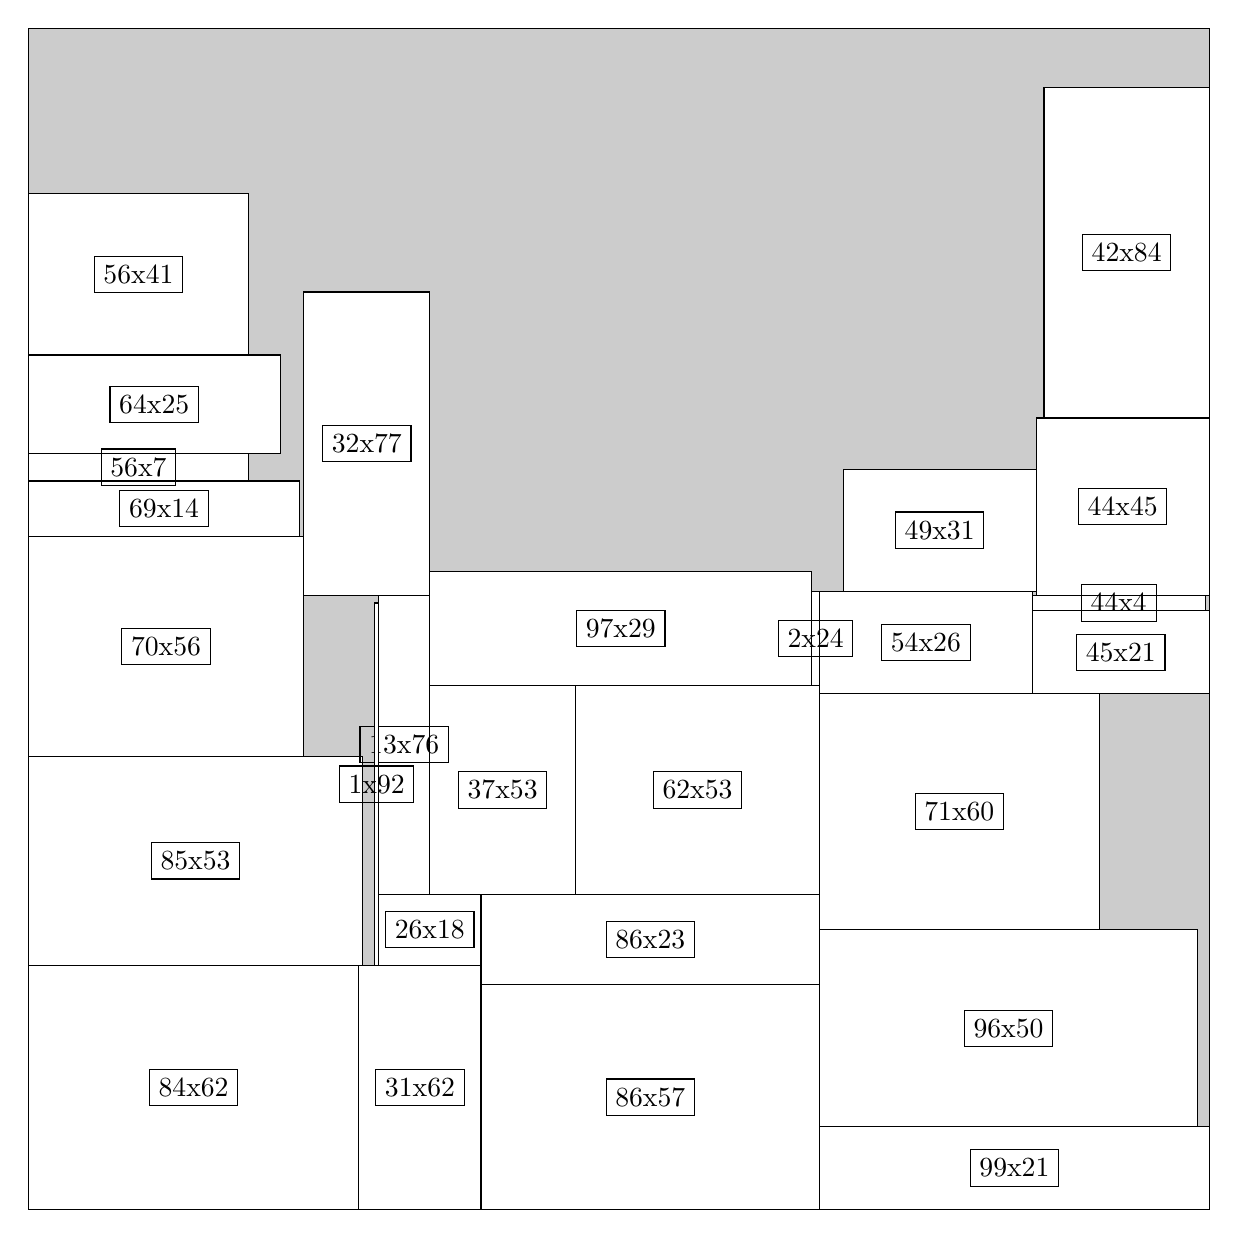
\begin{tikzpicture}[shorten >=1pt,scale=1.0,every node/.style={scale=1.0},->]
\tikzstyle{vertex}=[circle,fill=black!25,minimum size=14pt,inner sep=0pt]
\filldraw[fill=gray!40!white, draw=black] (0,0) rectangle (15.0,15.0);
\foreach \name/\x/\y/\w/\h in {84x62/0.0/0.0/4.2/3.1,86x57/5.75/0.0/4.3/2.85,96x50/10.05/1.05/4.800000000000001/2.5,85x53/0.0/3.1/4.25/2.6500000000000004,71x60/10.05/3.5500000000000003/3.5500000000000003/3.0,70x56/0.0/5.75/3.5/2.8000000000000003,62x53/6.95/4.0/3.1/2.6500000000000004,97x29/5.1000000000000005/6.65/4.8500000000000005/1.4500000000000002,32x77/3.5/7.800000000000001/1.6/3.85,56x41/0.0/10.850000000000001/2.8000000000000003/2.0500000000000003,99x21/10.05/0.0/4.95/1.05,44x45/12.8/7.800000000000001/2.2/2.25,86x23/5.75/2.85/4.3/1.1500000000000001,37x53/5.1000000000000005/4.0/1.85/2.6500000000000004,31x62/4.2/0.0/1.55/3.1,64x25/0.0/9.600000000000001/3.2/1.25,49x31/10.350000000000001/7.8500000000000005/2.45/1.55,54x26/10.05/6.550000000000001/2.7/1.3,13x76/4.45/4.0/0.65/3.8000000000000003,69x14/0.0/8.55/3.45/0.7000000000000001,42x84/12.9/10.05/2.1/4.2,45x21/12.75/6.550000000000001/2.25/1.05,26x18/4.45/3.1/1.3/0.9,56x7/0.0/9.25/2.8000000000000003/0.35000000000000003,44x4/12.75/7.6000000000000005/2.2/0.2,1x92/4.4/3.1/0.05/4.6000000000000005,2x24/9.950000000000001/6.65/0.1/1.2000000000000002}
\filldraw[fill=white!40!white, draw=black] (\x,\y) rectangle node[draw] (\name) {\name} ++(\w,\h);
\end{tikzpicture}


w =84 , h =62 , x =0 , y =0 , v =5208
\par
w =86 , h =57 , x =115 , y =0 , v =4902
\par
w =96 , h =50 , x =201 , y =21 , v =4800
\par
w =85 , h =53 , x =0 , y =62 , v =4505
\par
w =71 , h =60 , x =201 , y =71 , v =4260
\par
w =70 , h =56 , x =0 , y =115 , v =3920
\par
w =62 , h =53 , x =139 , y =80 , v =3286
\par
w =97 , h =29 , x =102 , y =133 , v =2813
\par
w =32 , h =77 , x =70 , y =156 , v =2464
\par
w =56 , h =41 , x =0 , y =217 , v =2296
\par
w =99 , h =21 , x =201 , y =0 , v =2079
\par
w =44 , h =45 , x =256 , y =156 , v =1980
\par
w =86 , h =23 , x =115 , y =57 , v =1978
\par
w =37 , h =53 , x =102 , y =80 , v =1961
\par
w =31 , h =62 , x =84 , y =0 , v =1922
\par
w =64 , h =25 , x =0 , y =192 , v =1600
\par
w =49 , h =31 , x =207 , y =157 , v =1519
\par
w =54 , h =26 , x =201 , y =131 , v =1404
\par
w =13 , h =76 , x =89 , y =80 , v =988
\par
w =69 , h =14 , x =0 , y =171 , v =966
\par
w =42 , h =84 , x =258 , y =201 , v =3528
\par
w =45 , h =21 , x =255 , y =131 , v =945
\par
w =26 , h =18 , x =89 , y =62 , v =468
\par
w =56 , h =7 , x =0 , y =185 , v =392
\par
w =44 , h =4 , x =255 , y =152 , v =176
\par
w =1 , h =92 , x =88 , y =62 , v =92
\par
w =2 , h =24 , x =199 , y =133 , v =48
\par
\newpage


\end{document}